%!TEX root=../GaugeCNNTheory.tex


\subsection{Quotient kernel fields}
\label{sec:quotient_kernel_fields}


Theorem~\ref{thm:isometry_equivariant_kernel_field_trafos} showed that the isometry equivariance of a kernel field transform requires the invariance of the corresponding kernel field.
Since the invariance constraint implies kernels to be shared over orbits as visualized in Fig.~\ref{fig:isom_invariant_kernel_field_multiple_orbits}, the mathematical description of such invariant kernel fields is redundant:
a single kernel at one orbit representative is sufficient to reconstruct the kernel field on the whole orbit.
In Section~\ref{sec:quotient_kernels_stabilizers} we derive equivalent, reduced descriptions of invariant kernel fields in terms of kernels on orbit representatives.
These representative kernels are themselves constrained by the action of the stabilizer subgroup of the orbit representative.
We propose a (unique) lifting from representative kernels to invariant kernel fields, which establishes an isomorphism between both descriptions.
This lifting isomorphism suggest a way of parameterizing and constructing isometry equivariant kernel field transforms in an implementation.
Before deriving these results in Section~\ref{sec:quotient_kernels_stabilizers}, the following Section~\ref{sec:isom_quotients} sets up the mathematical framework.

The derivations and results of this section are close in spirit to the theory of \emph{steerable CNNs on homogeneous spaces}~\cite{Cohen2018-intertwiners,Cohen2019-generaltheory},
however, we generalize their results from homogeneous spaces to general manifolds.
When sticking to homogeneous spaces $M$, we prove that isometry equivariant kernel field transforms are equivalent to $\GM$-convolutions.





\subsubsection{Isometry induced quotient spaces}
\label{sec:isom_quotients}


The action of a symmetry group on a space partitions it into orbits, defined as the sets of all points which are connected by the group action.
The space of such orbits is the \emph{quotient space} w.r.t. this group action.
In the following we will discuss the quotient spaces arising from the actions of some isometry group $\I \leq \IsomGM$ both on the manifold and on the fiber bundles.
These definitions will later allow us to share weights over orbits by acting with isometries on kernels.



\paragraph{Manifold quotients:} 

Any point $p\in M$ traces out an \emph{orbit}
\begin{align}\label{eq:orbit_Ip}
    \I.p \,:=\, \big\{ \phi(p) \;\big|\; \phi \in\I \,\big\}\ \subseteq\, M \,,
\end{align}
which is defined as the set of all points reached by acting on $p$ with any isometry in $\I \leq \IsomM$.
One can easily check that the relation ``$p$ and $q$ are elements of the same orbit'' is an equivalence relation (see footnote \ref{footnote:equiv_rel}) and thus \emph{partitions} the manifold as visualized in Fig.~\ref{fig:isom_egg_quotient_M}.
The quotient space
\begin{align}\label{eq:quotientspace_IM}
    \IM \, :=\, \big\{ \I.p \,\big|\, p\in M \big\}
\end{align}
with respect to this equivalence relation is the space of all orbits, that is, each element of $\IM$ corresponds to a full orbit in~$M$.%
\footnote{%
    We write $\IM$ as a left quotient since $\I$ acts on $M$ from the left.
}
The corresponding \emph{quotient map}
\begin{align}\label{eq:quotientmap_QM}
    \QM: M\to\IM,\ \ p\mapsto \I.p
\end{align}
identifies a point $p \in M$ with its orbit $\I.p \in \IM$.
For each orbit one can select an arbitrary \emph{orbit representative}, formally determined by a \emph{section}
\begin{align}\label{eq:section_rM}
    \rM: \IM\to M \quad \textup{such that}\quad \QM\circ\rM = \id_{\IM} \,,
\end{align}
where the last condition ensures that the representative $\rM(\I.p)$ is indeed an element of the orbit $\I.p$.
One is often interested in continuous (or smooth) sections, however, these do in general not exist.
We will therefore in the following \emph{not} demand the orbit representatives to be chosen continuously and make up for this shortcoming post-hoc if necessary.
As usual for sections, they are in general only right inverses of the quotient map but not left inverses, that is, $\rM\circ\QM \neq \id_M$.
This is visualized by a commutative diagram
\begin{equation}
\begin{tikzcd}[row sep=3em, column sep=4.5em]
      \IM
            \arrow[r, "\rM"]
            \arrow[rr, rounded corners, to path={ 
                  -- ([yshift=-3.ex]\tikztostart.south) 
                  --node[below, pos=.5]{\small$\id_{\IM}$} ([yshift=-3.ex]\tikztotarget.south) 
                  -- (\tikztotarget.south)
                  }]
    & M
            \arrow[r, "\QM"]
    & \IM
\end{tikzcd}
\end{equation}
similar to that in Eq.~\eqref{cd:section_proj_idM} and a non-commutative diagram
\begin{equation}
\begin{tikzcd}[row sep=3em, column sep=4.5em,
               execute at end picture={
                    \node [] at (-.04, -.46) {$\noncommutative$};
                    }]
      M
            \arrow[r, "\QM"]
            \arrow[rr, rounded corners, to path={ 
                  -- ([yshift=-3.5ex]\tikztostart.south) 
                  --node[below, pos=.5]{\small$\id_M$} ([yshift=-3.5ex]\tikztotarget.south) 
                  -- (\tikztotarget.south)
                  }]
    & \IM
            \arrow[r, "\rM"]
    & M
\end{tikzcd}
\end{equation}
similar to that in Eq.~\eqref{cd:section_proj_noncommutative}.
The individual fibers $\preim{\QM}\mkern-4mu(\I.p) = \I.p \subseteq M$ of the quotient map $\QM$ are given by the orbits themselves.
Note that $M\xrightarrow{\QM}\IM$ is in general \emph{not} a fiber bundle since the orbits are not necessarily homeomorphic to each other and can therefore not be locally trivialized with a shared typical fiber $F$, as required by the commutative diagram in Eq.~\eqref{cd:trivialization_general_intro}.
Each orbit therefore has an own \emph{type} which is in close relation to the stabilizer subgroups of the points on that particular orbit.
The \emph{stabilizer subgroup}
\begin{align}
    \Stab{p} \,:=\, \big\{ \xi \in \I \,\big|\, \xi(p)=p \big\} \ \leq\ \I
\end{align}
of a point $p\in M$ is thereby defined as that subgroup of the isometry group which leaves $p$ fixed.
In terms of the stabilizer subgroup, it holds that the orbit of a point is identified with
\begin{align}
    \I.p \ \cong\ \I/\Stab{p} \,.
\end{align}
To see this claim, let $f_p: \I \to \I.p,\ \phi \mapsto \phi(p)$ for some $p\in M$ and observe that $f_p(\phi\circ\xi) = \phi\circ\xi(p) = \phi(p) = f_p(\phi)$ for any $\xi\in\Stab{p}$.
It can easily be shown that indeed $\preim{f_p}\!\! \big(\phi(p)\big) = \phi.\Stab{p}$ is a coset of the stabilizer subgroup of $p$ and thus that $f_p$ establishes the claimed isomorphism $\I.p \,\cong\, \I/\Stab{p}$.

\begin{figure}
    \centering%
    \subcaptionbox{\small Quotient map and orbit representatives for $M$.%
        \label{fig:isom_egg_quotient_M}}%
        [.44\linewidth][l]{%
            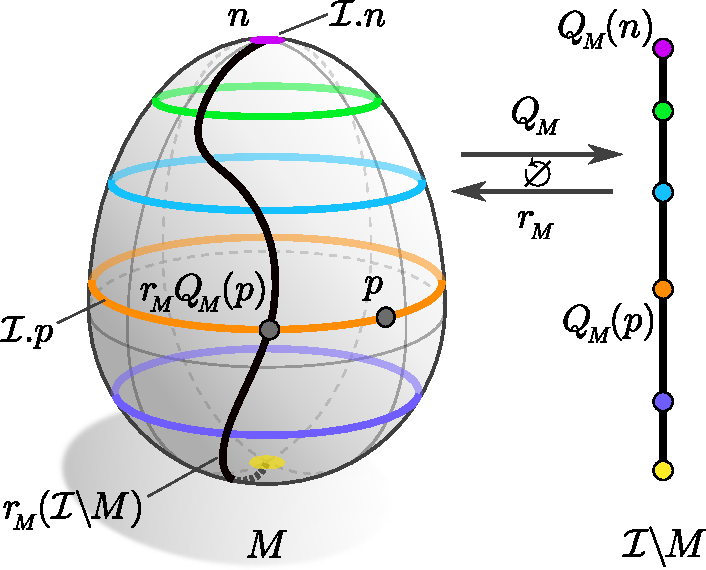
\includegraphics[width=.43\textwidth]{figures/isometry_egg_quotient_M.pdf}%
            \vspace*{1ex}%
        }%
    \hfill%
    \subcaptionbox{\small Quotient map and orbit representatives for $\TM$.%
        \label{fig:isom_egg_quotient_TM}}%
        [.5\linewidth][r]{%
            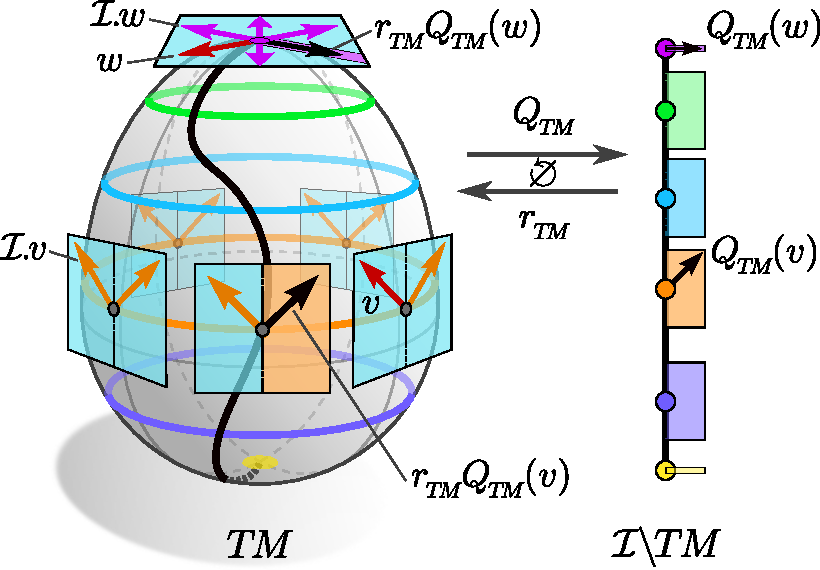
\includegraphics[width=.5\textwidth]{figures/isometry_egg_quotient_TM.pdf}%
            \vspace*{1ex}%
        }%
    \caption{\small%
        Quotient maps $\QM$ and $\QTM$ and orbit representatives (sections) $\rM$ and $\rTM$ for the actions of the isometry group $\I=\O2$ on the manifold~$M$ in Fig.~\ref{fig:isom_egg_quotient_M} and on the tangent bundle $\TM$ in Fig.~\ref{fig:isom_egg_quotient_TM}.
        A detailed description of both visualizations is given in the main text.
    }%
    \label{fig:isom_egg_quotient_main}%
\end{figure}

To make these constructions more intuitive, consider the example in Fig.~\ref{fig:isom_egg_quotient_M} with $\I \cong \O2$.
The orbits $\I.n = \{n\}$ and $\I.s = \{s\}$ of the north and south pole are just points, which are fixed by $\I$.
This agrees with, for instance, $\I.n \cong \I/\Stab{n} = \I/\I \cong \{n\}$ since $\Stab{n}=\I$ coincides with the full isometry group.
For any other point $p\in M$, the orbits $\I.p$ are circles.
We have reflections $\Stab{p} \cong \Flip$ (flipping over $p$) as stabilizer subgroup and thus indeed get the circle $\I/\Stab{p} \cong \O2/\Flip \cong S^1$ as orbit type.
The quotient map $\QM:M\to\IM$ sends points $q\in M$ to their orbits $\QM(q) = \I.q$ in the quotient space $\IM$, shown on the right.
Since the orbits can be traversed from the north to the south pole, the quotient space $\IM$ has the topology of a line segment.
The section $\rM:\IM\to M$ picks one representative point $\rM(o) \in M$ for any orbit $o \in \IM$.
In general, this orbit representative does not recover a projected point.
For instance, we have that $\rM\QM(p) \neq p$.
One can interpret the section as embedding the quotient space $\IM$ into the manifold, shown as the black line $\rM(\IM)$ from the north to the south pole.





\paragraph{Bundle quotients:}

Since the isometry group acts not only on the manifold itself but via pushforwards also on the associated bundles, these bundles are in a similar manner partitioned into orbits.
To keep the discussion general, we are in the following considering a generic associated bundle $E\xrightarrow{\pi_E} M$, which could stand for $\TM$, $\FM$, $\GM$, $\A$ or $\Hom(\Ain,\Aout)$.
We denote elements of the total space as $e\in E$ and let $\dphiE$ be the pushforward of $\phi$ on $E$ as introduced in Section~\ref{sec:isom_action_bundles}.
The orbit of an element of the bundle is then in analogy to Eq.~\eqref{eq:orbit_Ip} given by
\begin{align}\label{eq:bundle_orbit_def}
    \I.e \:=\ \big\{ \dphiE(e) \,\big|\, \phi\in\I \big\}
\end{align}
while the quotient space, consisting of bundle orbits, is analogously to Eq.~\eqref{eq:quotientspace_IM} defined as
\begin{align}
    \IE \:=\ \big\{ \I.e \,\big|\, e\in E \big\} \,.
\end{align}
Similar to before, the (canonical) quotient map sends bundle elements to their orbit:
\begin{align}
    \QE: E\mapsto\IE,\ \ e\mapsto\I.e
\end{align}
We define a (uniquely determined) projection map 
\begin{align}\label{eq:quotient_projection_piIE}
    \piIE\!:\, \IE \to \IM, \quad \QE(e) \mapsto \QM \circ \piE(e)
\end{align}
between the bundle quotients and manifold quotient as visualized in the following commutative diagram:
\begin{equation}\label{cd:QE_IE}
\begin{tikzcd}[column sep=50pt, row sep=30, font=\normalsize]
    \IE     \arrow[d, "\piIE"']
    &
    E       \arrow[l, "\QE"']
            \arrow[d, "\piE"]
    \\
    \IM
    &
    M       \arrow[l, "\QM"]
\end{tikzcd}
\end{equation}
Note that the definition in Eq.~\eqref{eq:quotient_projection_piIE} does not depend on the particular choice of orbit representative since for any other $\dphiE(e) \in \QE(e)$ we obtain the same result:
$    \QM \circ \piE \circ \dphiE(e)
\,=\,\QM \circ \phi \circ \piE(e)
\,=\,\QM \circ \piE(e) .
$
Orbit representatives are formally determined by a choice of section
\begin{align}\label{eq:bundle_quotient_section_def}
    \rE: \IE\to E \quad \textup{such that}\quad \QE\circ\rE = \id_{\IE} \,,
\end{align}
which we again do not demand to be continuous.
However, for convenience we demand the representatives of bundle orbits to lie above the representatives $\rM(\IM)$ in the base space, that is, to satisfy
\begin{align}\label{eq:bundle_quotient_section_isom}
    \piE \circ \rE \ =\ \rM \circ \piIE
\end{align}
as shown in the commutative diagram below:
\begin{equation}
\begin{tikzcd}[column sep=50pt, row sep=30, font=\normalsize]
    \IE     \arrow[d, "\piIE"']
            \arrow[r, "\rE"]
    &
    E       \arrow[d, "\piE"]
    \\
    \IM     \arrow[r, "\rM"']
    &
    M
\end{tikzcd}
\end{equation}


The stabilizer subgroup of a bundle element $e\in E$ is defined as
\begin{align}
    \Stab{e} \,:=\, \big\{ \xi \in \I \;\big|\; \dxiE e=e \big\} \ \leq\ \Stab{\piE(e)}\ \leq\ \I \,.
\end{align}
It is necessarily a subgroup of the stabilizer subgroup $\Stab{\piE(e)}$ of the point $\piE(e)$ in the base space, which is easily seen by
$ \ \xi \in \Stab{e}                        \ \Leftrightarrow\ 
    \dxiE e = e                             \ \Rightarrow\ 
    \piE(\dxiE e) = \xi\, \piE(e) = \piE(e) \ \Leftrightarrow\ 
    \xi \in \Stab{\piE(e)} .
$
As before, the relation $\I.e \cong \I/\Stab{e}$ holds.


We extend our example from Fig.~\ref{fig:isom_egg_quotient_M} by considering the action of $\I\cong\O2$ on the tangent bundle $\TM$ of the egg $M$ in Fig.~\ref{fig:isom_egg_quotient_TM}.
The orbit (violet) of a non-zero vector $0\neq w\in T_nM$ (red) at the north pole~$n$ describes a circle in $T_nM$.
This is consistent with $\I.w \cong \I/\Stab{w} \cong \O2/\Flip \cong S^1$ since such a vector is stabilized by reflections $\Stab{w} \cong \Flip$ along its axis.
The orbit of $0\in T_nM$ is a single point in $\TM$, which is stabilized by any isometry.
Any other vector $v\in\TpM$ (red), living in a tangent space at a point $p\in M$ different from the poles, is by the action of the isometry group rotated and reflected to other tangent spaces $\TphipM$ on the orbit $\I.p$ of $p$.
The orbit $\I.v$ (orange) of any such vector, if not pointing exactly to the north or south, is given by an eastward and a westward pointing copy of the vector in each of the tangent spaces over $\I.p$.
We have $\Stab{v}=\{e\}$ for such vectors and indeed the orbit $\I.v \cong \I/\Stab{v} \cong \O2/\{e\}$ is homeomorphic to $\O2$ (or two circles).
Vectors $v'\in\TpM$ which do point exactly north- or southwards are stabilized by reflections over the axis which they define, that is, $\Stab{v'} \cong \Flip$.
Their orbit is homeomorphic to a circle $\I.v' \cong \I/\Stab{v'} \cong \O2/\Flip \cong S^1$.

The quotient map $\QTM: \TM \to \ITM$ projects the tangent bundle to the bundle quotient $\ITM$, shown in the right half of Fig.~\ref{fig:isom_egg_quotient_TM}.
To understand its structure, we consider all qualitatively different cases:
Firstly, note that the orbits of vectors at the poles correspond to circles of a certain radius, such that the set of such orbits forms a line $\piIE^{-1}(\I.n) \cong \R^+$ (pink ray under the black arrow).
Similarly, the orbits of vectors at any other point $p\in M$ intersect all tangent spaces $\TphipM$ over $\I.p$ in two reflections and therefore form a half plane $\piIE^{-1}(\I.p) \cong \R\times\R^+$ (orange).
The section $\rTM: \ITM \to \TM$ sends each bundle quotient element to some representative in $\TM$.
By the requirement in Eq.~\eqref{eq:bundle_quotient_section_isom}, these representatives are required to lie in the same fiber over the representatives $\rM(\IM)$ of the manifold quotient $\IM$, shown as the black line.
For instance, $v\in\TpM$ (red) is by the quotient map sent to $\QTM(v)\in \ITM$ (black).
The section represents $\QTM(v)$ by $\rTM\QTM(v)$ (also black), which is an element of $T_{\rM\QM(p)}M$ and does in general differ from $v$.



















\subsubsection{Quotient representative kernel fields and stabilizer constraints}
\label{sec:quotient_kernels_stabilizers}


To motivate the construction of quotient representative kernel fields and stabilizer constraints, consider the more explicit formulation
\begin{align}\label{eq:isom_invariant_kernel_constraint_explicit}
    \dphiHom \!\circ \Kp \circ \dphiTMinv \,=\ \Kphip \qquad \forall\, p\in M,\ \  \phi\in\I \,.
\end{align}
of the isometry invariance constraint from Def.~\ref{dfn:isometry_invariant_kernel_fields}, which follows by writing out Eq.~\eqref{eq:kernel_constraint_isom_full_1} for any point~${p\in M}$ individually.
This formulation emphasizes that the constraint leads to \emph{shared weights along the manifold orbits} $\I.p \in \IM$ as visualized in Figs.~\ref{fig:isom_invariant_kernel_field_multiple_orbits} and~\ref{fig:isom_invariant_kernel_field_quotient}.
It implies that the kernel $\Kr$ at an \emph{arbitrary representative point} $r = \rM(o)$ of any orbit $o = \I.r$ fully specifies the kernel field on the rest of the orbit, i.e. at all points $\phi(r)$ where $\phi\in\I$.
The kernel $\Kr$ at the representative point $r$ is itself constrained by the stabilizer subgroup of~$r$:
\begin{align}\label{eq:stab_constraint_teaser}
    \dxiHom \!\circ \Kr \circ \dxiTMinv \,=\ \Kr \qquad \forall\, \xi\in\Stab{r} \,.
\end{align}
This implies that any isometry invariant kernel field can be parameterized in terms of a field of kernels on manifold orbit representatives $r \in \rM(\IM)$ which satisfy Eq.~\eqref{eq:stab_constraint_teaser}.

In case that the stabilizer subgroup at $r$ happens to be non-trivial, the stabilizer constraint in Eq.~\eqref{eq:stab_constraint_teaser} implies further symmetries of the kernel $\Kr$ at~$r$ itself.
For instance, in the example in Fig.~\ref{fig:isom_invariant_kernel_field_quotient} one has the stabilizer subgroup ${\Stab{r} \cong \Flip}$ on the highlighted orbit, enforcing a reflectional symmetry of the kernels.
Such stabilizer symmetries allows to compress the description of isometry invariant kernel fields further:
it turns out to be sufficient to know the values $\K(w)$ of the kernel field on the tangent bundle quotient representatives $w \in \rTM(\ITM) \subseteq \TM$ only.
In Fig.~\ref{fig:isom_invariant_kernel_field_quotient} this corresponds to knowing the kernel values on the orange highlighted half space, from which the full field on the orbit can be reconstructed by the reflectional and rotational symmetries in $\I\cong\O2$.



Theorem~\ref{thm:tangent_quotient_repr_kernel_fields} below makes the latter claim precise by proving that the space $\KIfull$ of isometry invariant kernel fields is isomorphic to a space $\KIquot$ of kernel fields on tangent bundle orbit representatives $\rTM(\ITM)$.
$\KIquot$~is characterized by maximally reduced constraints and thus encodes the kernel fields in $\KIfull$ in a non-redundant way.
It can therefore be viewed as the distilled degrees of freedom contained in $\KIfull$.
In~Theorem~\ref{thm:manifold_quotient_repr_kernel_fields} we formulate a third isomorphic space $\KIquothat$, which equivalently describes isometry invariant kernel fields in terms of the stabilizer subgroup constrained kernels $\Kr$ from Eq.~\eqref{eq:stab_constraint_teaser}.
While the formulation of isometry invariant kernel fields in terms of $\KIquothat$ involves stronger constraints than that in terms of $\KIquot$, it might be more convenient for implementations, since it describes kernels on full tangent spaces instead of kernels on quotients of tangent spaces.

\begin{SCfigure}
    \centering
    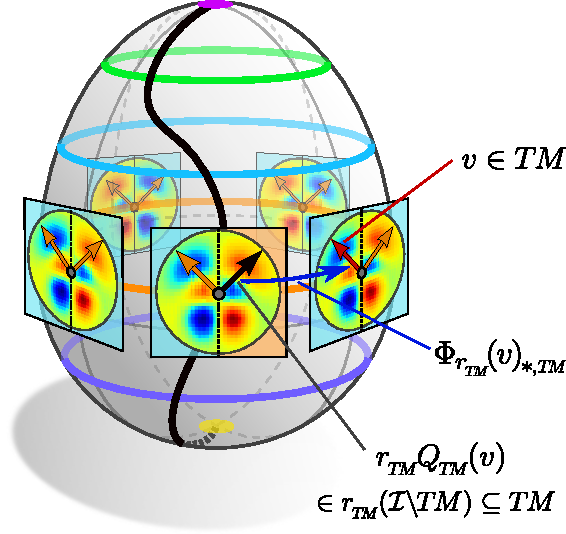
\includegraphics[width=.51\columnwidth]{figures/isometry_egg_quotient_kernel.pdf}
    \captionsetup{width=1.\textwidth}
    \hfill
    \caption{\small
        Visualization of an isometry invariant kernel field, Def.~\ref{dfn:isometry_invariant_kernel_fields}, and its full reconstruction from kernels on quotient representatives only.
        In contrast to Fig~\ref{fig:isom_invariant_kernel_field_multiple_orbits}, we assume here an isometry group $\I = \O2$ instead of $\SO2$.
        The visualized kernels therefore have a reflectional symmetry, which is enforced by the stabilizer subgroups $\Stab{p} \!\cong\! \Flip$ of points on the orbit $\I.\piTM(v)$.
        Due to its symmetry, the full kernel field $\K: \TM\to \Hom(\Ain,\Aout)$ can be reconstructed from its restriction to the bundle quotient representative $\rTM(\ITM) \subseteq \TM$; see Theorem~\ref{thm:tangent_quotient_repr_kernel_fields}.
        For instance, the shown kernels are fully determined by the partial kernel on the orange half space.
        The reconstruction at $v\in \TM$ is done by evaluating the quotient representative kernel at $\rTM\QTM(v) \in \rTM(\ITM)$ and pushing the kernel via the reconstruction isometry $\PhirNoArg(v) \in \I$, defined in Eq.~\eqref{eq:reconstruction_isometry}, back to $v$.
        We want to mention that the visualized \emph{anti}symmetric kernels would result when mapping between feature fields of even and odd parity, while kernels between feature fields of the same parity would be symmetric.
        }
    \label{fig:isom_invariant_kernel_field_quotient}
\end{SCfigure}



\paragraph{Reconstruction isometries:}
In order to reconstruct full invariant kernel fields in $\KIfull$ from single kernels on orbit representatives, the representative kernels need to be redistributed over the full manifold by applying the kernel pushforward in Eq.~\eqref{eq:isom_invariant_kernel_constraint_explicit} with $p=r$ fixed to the chosen representative points.
For the kernel reconstruction at some point $q\in M$, this requires some isometry $\phi$ which maps the orbit representative $\rM\QM(q) \in \rM(\IM) \subseteq M$ back to $q\in M$, that is, which satisfies $\phi\big(\rM\QM(q)\big) = q$.
To make this more precise, recall that kernel fields $\K: \TM\to \Hom(\Ain,\Aout)$ are defined as maps with domain $\TM$, encoding the \emph{kernel alignments} in addition to their position.
We therefore need to consider more specific isometries which push tangent bundle orbit representatives $\rTM\QTM(v) \in \rTM(\ITM) \subseteq \TM$ back to vectors $v \in \TM$.
These \emph{reconstruction isometries} are defined by:%
\footnote{
    Since the sections $\rTM$ are in general not continuous, $\PhirNoArg$ can in general not be demanded to be continuous either.
}
\begin{align}\label{eq:reconstruction_isometry}
    \PhirNoArg: \TM \to \I \quad\textup{such that}\quad \dPhirTM{v}\, \rTM\mkern1mu \QTM(v) = v \quad \forall\, v\in \TM
\end{align}
We recommend to consult Fig.~\ref{fig:isom_invariant_kernel_field_quotient} to get an intuition for the reconstruction isometries:
graphically, $\Phir{v}$ is defined as \emph{any} isometry which pushes the black vector $\rTM\QTM(v)$ on the orange orbit $\I.v$ back to the red vector $v$ on the same orbit.
Note that $\PhirNoArg$ is only unique up to the stabilizer subgroups of the orbit representatives since for any $\xi\in \Stab{\rTM\QTM(v)}$ it follows that $\Phir{v} \xi$ satisfies the defining constraint in Eq.~\eqref{eq:reconstruction_isometry} as well:%
\footnote{\label{footnote:ambiguity_reconstruction_isometry}:%
    Furthermore, the defining constraint on $\PhirNoArg$ is fulfilled when \emph{left} multiplying $\Phir{v}$ with any $\zeta\in\Stab{v}$.
    This does, however, not add any new degrees of freedom since $\Stab{v} \cong \Stab{\rTM\QTM(v)}$ and
    $\zeta\,\Phir{v} = \Phir{v} \big[\Phir{v}^{-1} \zeta \Phir{v}\big] =: \Phir{v} \widetilde{\zeta}$
    with $\widetilde{\zeta} \in \Stab{\rTM\QTM(v)}$.
}
$\big[ \Phir{v}\, \xi\, \big]_{\!*,\scalebox{.58}{$T\mkern-1.5muM$}}\mkern2mu \rTM\QTM(v) = \dPhirTM{v}\, \rTM\QTM(v) = v$.
All of the following constructions are shown to be independent from this ambiguity.
The action of reconstruction isometries on the base space~$M$ follows by applying the tangent bundle projection to both sides of the defining constraint in Eq.~\eqref{eq:reconstruction_isometry}:
\begin{alignat}{3}\label{eq:reconstruction_isometry_basespace}
    \qquad\qquad\qquad
    \piTM(v)
    \ &=\ \piTM \dPhirTM{v}\, \rTM\, \QTM(v)
        \qquad\quad && \big( \textup{\small Def. of $\PhirNoArg\,$, Eq.~\eqref{eq:reconstruction_isometry} } \big) \notag \\
    \ &=\ \Phir{v}\, \piTM\, \rTM\, \QTM(v)
        \qquad\quad && \big( \textup{\small Pushforward is a bundle map, Eq.~\eqref{eq:pushfwd_bundle_automorphism} } \big) \notag \\
    \ &=\ \Phir{v}\, \rM\, \piITM\, \QTM(v)
        \qquad\quad && \big( \textup{\small Def. of bundle sections, Eq.~\eqref{eq:bundle_quotient_section_isom} } \big) \notag \\
    \ &=\ \Phir{v}\, \rM\, \QM\,  \piTM(v)
        \qquad\quad && \big( \textup{\small Def. of $\piIE\,$, Eq.~\eqref{cd:QE_IE} } \big)
\end{alignat}
A visual summary of the properties of $\PhirNoArg$, that is, its actions on $\TM$ and $M$, is given in the following commutative diagram
\begin{equation}
    \begin{tikzcd}[row sep=3.5em, column sep=6em]
        % ROW 1
        \TM
            \arrow[d, "\piTM"']
            \arrow[r, "\PhirNoArg \,\times\ \rTM \mkern-2mu\circ\mkern-2mu \QTM"]
            \arrow[rr, rounded corners, to path={ 
                    -- ([yshift=+5.5ex]\tikztostart.north) 
                    --node[above, pos=.5]{\small$\id_{\TM}$} ([yshift=+5.5ex]\tikztotarget.north) 
                    -- (\tikztotarget.north)
                    }]
        &[10ex]
        \I \times \rTM(\ITM)
            \arrow[r, "\ev"]
            \arrow[d, "\id_{\I} \times \piTM"']
        & \TM
            \arrow[d, "\piTM"]
        \\
        % ROW 2
          M
            \arrow[rr, rounded corners, to path={ 
                    -- ([yshift=-5.5ex]\tikztostart.south) 
                    --node[below, pos=.5]{\small$\id_M$} ([yshift=-5.5ex]\tikztotarget.south) 
                    -- (\tikztotarget.south)
                    }]
        &[10ex] \I \times \rM(\IM)
            \arrow[r, pos=.52, "\ev"']
        & M
    \end{tikzcd}
    \quad
\end{equation}
where the \emph{evaluation maps} $\ev$ are, overloading the notation, given by $\ev: \I\times  M \to  M,\ (\phi,p) \mapsto \phi(p)$ and $\ev: \I\times \TM \to \TM,\ (\phi,v) \mapsto \dphiTM(v)$, respectively.




\paragraph{Quotient representative kernel fields:}
As argued above, the symmetries which are present in an \mbox{isometry} \mbox{invariant} feature field $\K \in \KIfull$ should allow for its full reconstruction from its restriction ${\Krestr: \rTM(\ITM) \to \rHom(\IHom)}$ to tangent bundle orbit representatives $\rTM(\ITM) \subseteq \TM$.%
\footnote{
    In the following we might abbreviate $\Hom(\Ain,\Aout)$ and $\I\backslash \Hom(\Ain,\Aout)$ with $\Hom$ and $\IHom$, respectively.
}
To~construct a (unique) \emph{lift}~$\Lambda$ which recovers $\K = \Lambda(\Krestr)$ from $\Krestr$, we expand tangent vectors~$v$ in the domain of $\K$ via the reconstruction isometry $\PhirNoArg$ from Eq.~\eqref{eq:reconstruction_isometry} and make use of the invariance (equivariance) of the kernel field in Eq.~\eqref{eq:kernel_constraint_isom_full_1}.
This leads to:
\begin{align}\label{eq:lambda_construction}
    \K(v)
    \ &=\,\ \K\; \dPhirTM{v}\; \rTM\, \QTM (v) \notag \\
    \ &=\,\ \dPhirHom{v}\, \K\; \rTM\, \QTM (v) \notag \\
    \ &=\,\ \dPhirHom{v}\, \Krestr\, \rTM\, \QTM (v) \notag \\
    \ &=:\  \pig[ \Lambda\big(\Krestr\big) \pig] (v)
\end{align}
Note that this construction is well defined despite the ambiguity of $\PhirNoArg$ w.r.t. the right multiplication with elements in $\Stab{\rTM\QTM(v)}$.
This is easily seen by observing that for any $w \in \TM$, any $\xi \in \Stab{w}$ and any $\K \in \KIfull$ one has $\dxiHom \K(w) = \K(\dxiTM w) = \K(w)$, which implies that $\Stab{\K(w)} \geq \Stab{w}$, and thus that the final result does not depend on the particular choice of the ambiguous $\PhirNoArg$.


Since the lift $\Lambda$ recovers invariant kernel fields from their restriction to tangent bundle orbit representatives, it can be viewed as the \emph{inverse} map of the restriction (of invariant kernel fields).
This viewpoint implies that the lift establishes an \emph{isomorphism} $\Lambda: \KIquot \to \KIfull$ between the image of the restriction $\KIquot$, which we still need to characterize, and $\KIfull$:
\begin{equation}
    \begin{tikzcd}[row sep=3.5em, column sep=12.em]
        \KIquot
            \arrow[r, bend left=8, shift left=2pt, "\Lambda"]
        &
        \KIfull
            \arrow[l, bend left=8, shift left=2pt, "\Lambda^{-1} = (\,\cdot\,)|_{\rTM(\ITM)}"]
    \end{tikzcd}
\end{equation}

In order to characterize the space $\KIquot$ which makes $\Lambda$ to an isomorphism, it is sufficient to list the properties of restricted fields $\Q := \Krestr \in \KIquot$ for $\K \in \KIfull$:
\begin{itemize}[leftmargin=0.6cm]

\item[{\rule[2.2pt]{2pt}{2pt}}]
First of all, since $\Lambda^{-1}$ is given by the restriction of the domain to $\rTM(\ITM)$, it is clear that any $\Q \in \KIquot$ is required to be of the form $\Q: \rTM(\ITM) \to \rHom(\IHom)$.

\item[{\rule[2.2pt]{2pt}{2pt}}]
Secondly, the property of kernel fields to be bundle $M$-morphisms translates under the restriction $\Lambda^{-1}$ to the requirement on $\Q$ to satisfy $\piHom\circ\Q(w) = \piTM(w)$ for any $w\in \rTM(\ITM)$

\item[{\rule[2.2pt]{2pt}{2pt}}]
Thirdly, $\Q$ is required to satisfy the \emph{(vector) stabilizer constraint} $\dxiHom \Q(w) = \Q(w)$ for any representative vector $w \mkern-2mu\in\mkern-1mu \rTM(\ITM)$ and any $\xi \mkern-1mu\in\mkern-1mu \Stab{w}$.
This requirement is a residual from the invariance constraint in Eq.~\eqref{eq:kernel_constraint_isom_full_1}, surviving the restriction.
\\
It can be deduced by considering the full constraint $\dphiHom \Q\, \dphiTMinv(w) = \Q(w)$ for any $w \in \rTM(\ITM)$ and any isometry $\phi\in\I$ which additionally satisfies that $\dphiTM(w) \in \rTM(\ITM)$, i.e. that the pushforward $\dphiTM(w)$ stays within the restricted domain of~$\Q$.
Note that $\dphiTM(w) \in \I.w$ and that $\rTM(\ITM)$ intersects each orbit exactly once.
This implies that $\I.w \cap \rTM(\ITM) = \{w\}$ such that $\phi\in\I$ is required to satisfy $\dphiTM(w)=w$, that is, $\phi\in \Stab{w}$.
The claimed (vector) stabilizer constraint follows from these considerations.
\\
For an intuition we refer back to Fig.~\ref{fig:isom_invariant_kernel_field_quotient} where the black representative vector $w = \rTM\QTM(v)$ is stabilized only by the trivial isometry $\xi=\{e\}$, implying that the corresponding value of $\Q$ is unconstrained.
Vectors $w' \in \rTM(\ITM)$ which point exactly north- or southwards, i.e. which lie on the dashed reflection axis, are stabilized by reflections in $\Stab{w'}\cong\Flip$, implying a constraint on the corresponding kernel values.%
\footnote{
    The exact constraint depends on the action $\dxiHom$ on $\Hom(\Ain,\Aout)$, which depends on $\rhoHom$ and thus on $\rhoin$ and $\rhoout$.
    The visualized kernel in Fig.~\eqref{fig:isom_invariant_kernel_field_quotient} would correspond to $\rhoHom$ being the sign-flip (odd parity) representation of the reflection group, which enforces antisymmetric kernels.
    The antisymmetry requires $\Q$ to be constrained to $\Q(w') = -\Q(w') = 0$ for $w'$ on the reflection axis; cf. Table~\ref{tab:reflection_steerable_kernels}
}

\item[{\rule[2.4pt]{2pt}{2pt}}]
As a last requirement, $\Q$ needs to lift to a \emph{smooth} kernel field, that is, $\Lambda(\Q)$ is required to be smooth.
Unfortunately, the smoothness (or even continuity) of $\Lambda(\Q)$ does not automatically follow from the smoothness (continuity) of $\Q$ since $\Lambda$ is defined in terms of $\rTM$ and $\PhirNoArg$, which can in general not be demanded to be smooth (continuous).

\end{itemize}


Before summarizing and proving these claims rigorously in Theorem~\ref{thm:tangent_quotient_repr_kernel_fields} below, we give a visual overview of the relation between $\Q = \Krestr \in \KIquot$ and its lift $\K = \Lambda(\Q) \in \KIfull$ in terms of commutative diagrams
\begin{equation}
    \begin{tikzcd}[row sep=3.5em, column sep=6em]
        % ROW 1
        \TM
            \arrow[r, "\PhirNoArg \,\times\ \Q \mkern-2mu\circ\mkern-2mu \rTM \mkern-2mu\circ\mkern-2mu \QTM"']
            \arrow[rr, rounded corners, to path={ 
                    -- ([yshift=+3.5ex]\tikztostart.north) 
                    --node[above, pos=.5]{\small$\K = \Lambda(\Q)$} ([yshift=+3.5ex]\tikztotarget.north) 
                    -- (\tikztotarget.north)
                    }]
        &[10ex]
        \I \times \rHom(\IHom)
            \arrow[r, "\ev"']
        & \Hom
    \end{tikzcd}
    \qquad
\end{equation}
and
\begin{equation}
    \begin{tikzcd}[row sep=5em, column sep=7.5em]
        % ROW 1
        \TM
            \arrow[rd, pos=.6, "\rTM\circ\QTM"]
            \arrow[rrddd, "\piTM"']
            \arrow[rrrr, "\K = \Lambda(\Q)"]
        & &[-7em] &[-7em] &
        \Hom
            \arrow[ld, pos=.6, "\rHom\circ\QHom"']
            \arrow[llddd, "\piHom"]
        \\[-1em]
        % ROW 2
        & \rTM(\ITM)
            \arrow[rr, "\Q"]
            \arrow[rd, start anchor={[xshift=-1ex]}, "\piTM"']
        & &
        \mkern-3mu
        \rHom(\IHom)
            \arrow[ld, "\piHom"]
        \\
        % ROW 3
        & &
        \rM(\IM)
        \\
        % ROW 4
        & &
        M
            \arrow[u, pos=.6, "\rM \!\circ\mkern-1mu \QM"' description]
    \end{tikzcd}
\end{equation}
In the last diagram, the commutativity of the top square follows by inserting the definition of the lift, which yields
$\rHom\QHom \Lambda(\Q) = \rHom\QHom \dPhirHom{v} \Q\, \rTM\QTM = \Q\, \rTM\QTM$.
The commutative of the bottom left and right squares follows from Eqs.~\ref{eq:bundle_quotient_section_isom} and~\ref{eq:quotient_projection_piIE}.


\begin{thm}[Tangent quotient representative kernel fields]
\label{thm:tangent_quotient_repr_kernel_fields}
    The space of isometry invariant kernel fields $\KIfull$ from Def.~\ref{dfn:isometry_invariant_kernel_fields} is isomorphic to the space $\KIquot$ of (vector) stabilizer subgroup constrained kernel fields on tangent bundle quotient representatives, defined as:%
    \footnote{
        This definition of $\KIquot$ is in cyclic dependency with that of $\Lambda$ in Eq.~\eqref{eq:lifting_isomorphism_lambda}.
        This could be avoided on the expense of 1) having to define spaces $\widetilde{\KIquot}$ and $\widetilde{\KIfull}$ without smoothness requirements, in terms of which 2) $\widetilde{\Lambda}: \widetilde{\KIquot} \to \widetilde{\KIfull}$ could be defined, which would 3) allow to demand the smoothness requirements in $\KIquot$ in terms of $\widetilde{\Lambda}$.
    }
    \begin{align}\label{eq:KIquot_def}
        \KIquot :=\,
            \Big\{ \Q \mkern-2mu: \rTM(\ITM) \to \rHom(\IHom) \,\Big|\:& 
            \piHom \mkern-5mu\circ\mkern-1mu \Q = \piTM,\quad
            \Lambda(\Q)\ \textup{smooth}, \\ &
            \dxiHom \Q(w) = \Q(w) \ \ \ \forall\; w \mkern-2mu\in\mkern-1mu \rTM(\ITM),\ \xi \mkern-1mu\in\mkern-1mu \Stab{w}
            \!\Big\} \notag
    \end{align}
    The (unique) \emph{lifting isomorphism} $\Lambda: \KIquot \to \KIfull$ between both spaces is hereby given by
    \begin{align}\label{eq:lifting_isomorphism_lambda}
        \Lambda(\Q): \TM \to \Hom(\Ain,\Aout),\ \ \ 
        v \mapsto \big[ \Lambda(\Q) \big](v) \,:=\, \dPhirHom{v} \Q\; \rTM \QTM(v) \,.
    \end{align}
    Its inverse $\Lambda^{-1}: \KIfull \to \KIquot$ is given by the restriction of invariant kernel fields to the bundle quotient representatives $\rTM(\ITM) \subseteq \TM$:
    \begin{align}\label{eq:lifting_isomorphism_lambda_inv}
        \Lambda^{-1}(\K): \rTM(\ITM) \to \rHom(\IHom),\ \ \ 
        w \mapsto \big[ \Lambda^{-1}(\K) \big](w) \,:=\, \Krestr(w)
    \end{align}
\end{thm}
\begin{proof}
    In order to prove that $\Lambda: \KIquot \to \KIfull$ is an isomorphism, we need to show that
    \textit{1)} $\Lambda^{-1}$ is indeed an inverse of $\Lambda$, that
    \textit{2)} the defining properties of $\KIfull$ and $\KIquot$ are satisfied after lifting and restricting and that
    \textit{3)} the constructions do not depend on arbitrary choices.
    In order to not overload this section, we outsource the full proof to Appendix~\ref{apx:lifting_iso_proof}.
    The individual steps of the proof are listed below:
    \begin{itemize}[leftmargin=1.25cm]
        \item[\it 1\hspace{1pt}a)] $\Lambda \circ \Lambda^{-1} = \id_{\KIfull}$,
            that is, $\Lambda^{-1}$ is a right inverse of $\Lambda$
        \item[\it 1\hspace{1pt}b)] $\Lambda^{-1} \circ \Lambda = \id_{\KIquot}$,
            that is, $\Lambda^{-1}$ is a left inverse of $\Lambda$
        \item[\it 2\hspace{1pt}a)] $\piHom \mkern-5mu\circ\mkern-2mu \Lambda(\Q) = \piTM$ for any $\Q \in \KIquot$,
            that is, the lift $\Lambda(\Q)$ is a bundle $M$-morphism
        \item[\it 2\hspace{1pt}b)] ${\piHom \mkern-5mu\circ\mkern-2mu \Lambda^{-1}(\K) = \piTM}$ for any $\K \in \KIfull$
        \item[\it 2\hspace{1pt}c)] $\dphiHom \Lambda(\Q)\, \dphiTMinv = \Lambda(\Q)\ \ \forall \phi \in \I$,
            that is, $\Lambda(\Q)$ satisfies the full isometry invariance (equivariance) constraint
        \item[\it 2\hspace{1pt}d)] $\dxiHom \big[\Lambda^{-1}(\K)\big](w) = \big[\Lambda^{-1}(\K)\big](w) \ \ \
               \forall\; w \mkern-2mu\in\mkern-1mu \rTM(\ITM),\ \xi \mkern-1mu\in\mkern-1mu \Stab{w}$,\ 
            that is, $\Lambda^{-1}(\K)$ satisfies the stabilizer constraint
        \item[\it 3)] All constructions and proofs are independent from the particular choice of $\PhirNoArg$
    \end{itemize}
    The smoothness of lifted quotient representative kernel fields holds by definition.
\end{proof}
The arbitrariness in the choice of section $\rTM$ allows for different, isomorphic quotient kernel fields, expressed on different bundle quotient representatives.


Instead of maximally restricting the kernel field to bundle orbit representatives in $\rTM(\IM)$, one could choose to restrict the description to $\piTM^{-1}\big( \rM(\IM) \big)$ only, i.e. to \emph{complete tangent spaces} $T_rM$ for any $r\in \rM(\IM)$.
In Fig.~\eqref{fig:isom_invariant_kernel_field_quotient}, this would correspond to modeling the (reflection symmetric) kernel on the full tangent space shown in the front instead of only one half.
The requirements on such restricted kernels can be derived by following the same rationale as before and results in the constraint in Eq.~\eqref{eq:stab_constraint_teaser}.
We obtain a similar theorem to Theorem~\eqref{thm:tangent_quotient_repr_kernel_fields}:


\begin{thm}[Manifold quotient representative kernel fields]
\label{thm:manifold_quotient_repr_kernel_fields}
    The space of isometry invariant kernel fields $\KIfull$ from Def.~\ref{dfn:isometry_invariant_kernel_fields} is isomorphic to the space $\KIquothat$ of (manifold) stabilizer subgroup constrained kernel fields on the tangent spaces over manifold quotient representatives $\rM(\IM)$, defined as:
    \begin{align}\label{eq:KIquothat_def}
        \KIquothat :=\,
            \Big\{ \Qhat \mkern-2mu: \piTM^{-1}\big( \rM(\IM) \big) \to \piHom^{-1}\big( \rM(\IM) \big) \,\Big|\:& 
            \piHom \mkern-5mu\circ\mkern-1mu \Qhat = \piTM,\quad
            \widehat{\Lambda}(\Qhat)\ \textup{smooth}, \\ &
            \mkern-34mu
            \dxiHom \Qhat|_r\, \dxiTM^{-1} = \Qhat|_r \quad \forall\,\ r \mkern-2mu\in\mkern-1mu \rM(\IM),\,\ \xi \mkern-1mu\in\mkern-1mu \Stab{r}
            \!\Big\} \notag
    \end{align}
    The \emph{lifting isomorphism} $\widehat{\Lambda}: \KIquothat \to \KIfull$ is in terms of $\Lambda$ and a restriction defined as
    \begin{align}
        \widehat{\Lambda}\ :=\ \Lambda \circ (\,\cdot\,)\big|_{\rTM(\ITM)}
    \end{align}
    and therefore essentially agrees with $\Lambda$\textup{:}
    \begin{align}\label{eq:lifting_isomorphism_hat}
        \widehat{\Lambda}(\Qhat): \TM \to \Hom(\Ain,\Aout),\ \ \ 
        v \mapsto \big[ \widehat{\Lambda}(\Qhat) \big](v) \,:=\, \dPhirHom{v} \Qhat\; \rTM \QTM(v)
    \end{align}
    Its inverse $\widehat{\Lambda}^{-1}: \KIfull \to \KIquothat$ is given by the restriction of invariant kernel fields to 
    the tangent spaces over manifold quotient representatives:
    $\piTM^{-1}\big(\rM(\IM)\big) \subseteq \TM$:
    \begin{align}
        \widehat{\Lambda}^{-1}(\K): \piTM^{-1}\big(\rM(\IM)\big) \to \piHom^{-1}\big( \rM(\IM) \big),\ \ \ 
        \widehat{w} \mapsto \pig[ \widehat{\Lambda}^{-1}(\K) \pig](\widehat{w}) \,:=\, \K\big|_{\piTM^{-1}(\rM(\IM))}(\widehat{w})
    \end{align}
\end{thm}
\begin{proof}
    The proof is essentially analogous to that of Theorem~\ref{thm:tangent_quotient_repr_kernel_fields} with the slight difference that the stronger constraint
    $\dxiHom \Qhat|_r\, \dxiTM^{-1} = \Qhat|_r \quad \forall\,\ r \mkern-2mu\in\mkern-1mu \rM(\IM),\,\ \xi \mkern-1mu\in\mkern-1mu \Stab{r}$
    is required.
    Since it would not add much in addition to what is presented in Appendix~\ref{apx:lifting_iso_proof}, we omit the proof.
\end{proof}

The following commutative diagram shows the isomorphisms between the three equivalent descriptions of invariant kernel fields:
\begin{equation}
    \begin{tikzcd}[row sep=3.5em, column sep=13.em]
        \KIquot
            \arrow[r, bend left=7, shift left=2pt, "\Omega"]
            \arrow[rr, rounded corners, to path={ 
                    -- ([yshift=6.ex]\tikztostart.north) 
                    --node[above, pos=.49]{\small$\Lambda$} ([yshift=6.ex]\tikztotarget.north) 
                    -- (\tikztotarget.north)
                }]
        &
        \KIquothat
            \arrow[r, bend left=7, shift left=2pt, "\widehat{\Lambda}"]
            \arrow[l, bend left=7, shift left=2pt, "\Omega^{-1} = (\,\cdot\,)\big|_{\rTM(\ITM)}"]
        &
        \KIfull
            \arrow[l, bend left=7, shift left=2pt, "\widehat{\Lambda}^{-1} = (\,\cdot\,)\big|_{\piTM^{-1}(\rM(\IM))}"]
            \arrow[ll, rounded corners, to path={ 
                    -- ([yshift=-6.5ex]\tikztostart.south) 
                    --node[below, pos=.5]{\small$\Lambda^{-1} = (\,\cdot\,)\big|_{\rTM(\ITM)}$} ([yshift=-6.5ex]\tikztotarget.south) 
                    -- (\tikztotarget.south)
                }]
    \end{tikzcd}
\end{equation}










\paragraph{Relation to \emph{GM}-convolutions:}

The difference between $\IsomGM$-equivariant $\GM$-convolutions and general $\IsomGM$-equivariant kernel field transforms via $\IsomGM$-invariant kernel fields is that the former share $G$-steerable kernels over the whole manifold while the latter are only required to share $\Stab{p}$-steerable kernels over orbits $\IsomGM\!.p \in \IsomGMM$.
The requirement to share weights over the whole manifold is not strictly necessary but is -- supported by Occam's razor -- likely to be a good inductive bias in practice.
It can be viewed as an analog to the assumption that the same physical laws apply throughout the whole universe.

Assume now that $M$ is a \emph{homogeneous space} with respect to the action of some isometry group $\I \leq \IsomGM$, that is, for any two points $p,q\in M$ there is at least one isometry $\phi \in \I$ that connects both points, i.e. $q = \phi(p)$.
In this case there is only one single orbit $\I.p$, which is just $M$ itself, and the stabilizers $\Stab{p}$ of all points $p\in M$ coincide up to isomorphism.
The quotient space $\IM$ is a singleton which is represented by a single representative point $r = \rM(\IM)$ in~$M$.
By Theorem~\ref{thm:manifold_quotient_repr_kernel_fields}, the space of $\I$-invariant kernel fields is equivalently expressed by a kernel field on orbit representatives.
Since we have only a single representative point~$r$ for homogeneous spaces, the full isometry invariant kernel field is in this case equivalent to a single kernel on~$\TrM$.
This representative kernel is required to satisfy the stabilizer subgroup constraint in Eq.~\eqref{eq:KIquothat_def}.
Via the lifting isomorphism $\widehat{\Lambda}$ in Eq.~\eqref{eq:lifting_isomorphism_hat}, the representative kernel is shared over the whole manifold.

This sounds very similar to the definition of $\GM$-convolutions, which share a single, $G$-steerability constrained kernel over the whole manifold.
Theorem~\ref{thm:GM_conv_homogeneous_equivalence} below asserts that there is indeed an equivalence between convolutions and equivariant kernel field transforms on homogeneous spaces.
The coordinate free $\Stab{r}$-steerability from the stabilizer constraint thereby translates (non-canonically) to the $H$-steerability of template kernels, where $H \cong \Stab{r}$ with $H\leq G$ is an isomorphic representation of $\Stab{r}$ relative to some coordinatization.
One can view the isometry (sub)group $\I \leq \IsomGM$ as a principal $\Stab{r}$-bundle over $M$, whose (non-canonical) embedding into $\GM$ gives rise to a $H$-(sub)structure $\HM$ of~$\GM$.
The sharing of a $\Stab{r}$-steerable kernel via the lifting isomorphism, which operates per action of $\I$,
then corresponds exactly to the sharing of an $H$-steerable kernel over~$\HM$.
This implies that $\I$-equivariant kernel fields transforms on homogeneous spaces do indeed correspond to some $\HM$-convolution.
\begin{thm}[Equivariance on homogeneous \textit{M} implies convolution]
\label{thm:GM_conv_homogeneous_equivalence}
    Let $M$ be a manifold equipped with a $G$-structure~$\GM$.
    Assume that there is an isometry group $\I \leq \IsomGM$ which acts transitively on $M$, making it a \emph{homogeneous space}.
    Let $r\in M$ be an arbitrary representative point of $M$ and $\Stab{r} \leq \I$ its stabilizer.
    Then
    \begin{itemize}
        \item[\textit{1)}] There exists a $H$-(sub)structure $\HM \subseteq \GM$ on $M$ with:
            \begin{itemize}\setlength\itemsep{1ex}
                \item $H \cong \Stab{r} \leq \I$ is a subgroup of~$G \cap \O{d}$
                \item $\HM$ is an embedding of $\I$ (as principal $\Stab{r}$-bundle $\I \to \I/\Stab{r}$) into $\GM$, which is preserved by $\I$, that is, $\IsomHM = \I$
            \end{itemize}
        \item[\textit{2)}] Any $\I$-equivariant kernel field transform shares a single $H$-steerable kernel over the whole space $M$ and is equivalent to a $\HM$-convolution with that kernel.
    \end{itemize}
    The specific choice of $H$-structure depends on the chosen isomorphism $H \cong \Stab{r}$ but is irrelevant since $\I$-equivariant kernel field transforms can be equivalently expressed in any such choice.
\end{thm}
\begin{proof}
    The proof is found in Appendix~\ref{apx:homogeneous_equivalence_proof}.
\end{proof}
Our definition of isometry equivariant kernel field transforms is on homogeneous spaces essentially equivalent to the \emph{steerable convolutions on homogeneous spaces} as proposed by~\citet{Cohen2018-intertwiners}\cite{Cohen2019-generaltheory}.
The proven equivalence between isometry equivariant kernel field transforms and $\HM$-convolutions on homogeneous spaces therefore asserts that $\HM$-convolutions and steerable convolutions are essentially similar in this case.
However, while steerable convolutions are only defined on homogeneous spaces, $\HM$-convolutions generalize to general Riemannian manifolds.
More details on convolutions on homogeneous spaces are discussed in the related work Appendix~\ref{apx:homogeneous_conv}.
